\newpage
\subsubsection{Caso d'uso UC9.1: Annullamento Rinnovo API}
\label{UC9.1}
\begin{figure}[ht]
	\centering
	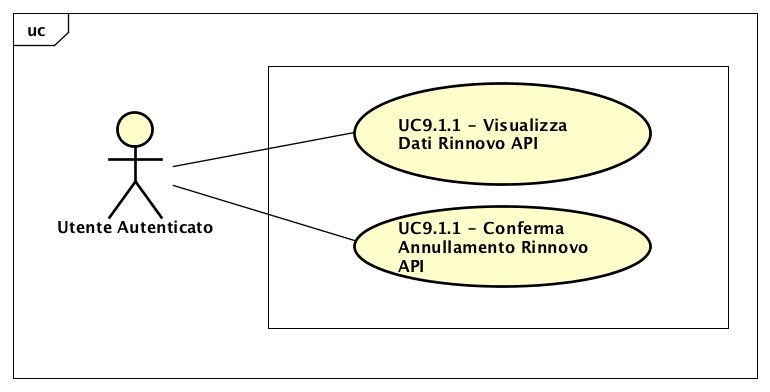
\includegraphics[scale=0.45]{UML/UC9_1.png}
	\caption{UC9.1: Annullamento Rinnovo API}
\end{figure}
\FloatBarrier
\renewcommand*{\arraystretch}{1.6}
\begin{longtable}{ l | p{11cm}}
	\hline
	\rowcolor{Gray}
	\multicolumn{2}{c}{UC9.1: Annullamento Rinnovo API} \\
	\hline
	\textbf{Attori} &Utente Autenticato, Amministratore APIMarket, Interfacce API Presente In APIMarket \\
	\textbf{Descrizione} & l'attore sceglie attraverso quale modalità interagire con le API acquistate \\
	\textbf{Pre-Condizioni} & l'attore ha scelto di gestire il rinnovo automatico di una API\\
	\textbf{Post-Condizioni}&l'attore ha effettuato le operazioni desiderate\\
	\textbf{Scenario Principale} & \begin{enumerate*}[label=(\arabic*.),itemjoin={\newline}]
		\item L'attore può visualizzare i dati riguardanti il rinnovo automatico di una API (UC9.1.1);
		\item L'attore può confermare l'annullamento del rinnovo automatico di una API (UC9.1.2)
	\end{enumerate*}\\
\end{longtable}

